\documentclass[10pt,twocolumn]{article}
\usepackage[a4paper,margin=0.75in,columnsep=0.28in]{geometry}
\usepackage[T1]{fontenc}
\usepackage{mathptmx}
\usepackage{microtype}
\usepackage{amsmath}
\usepackage{graphicx}
\graphicspath{{../assets/}{../eval/charts/}}
\usepackage{booktabs}
\usepackage{tabularx}
\usepackage{xcolor}
\usepackage[font=small,labelfont=bf,skip=4pt]{caption}
\usepackage{enumitem}
\usepackage{titlesec}
\usepackage[hidelinks]{hyperref}

\setlist{nosep,leftmargin=1.2em}
\titleformat{\section}{\normalfont\large\bfseries}{\thesection.}{0.5em}{}
\titleformat{\subsection}{\normalfont\normalsize\bfseries}{\thesubsection}{0.5em}{}
\titlespacing*{\section}{0pt}{9pt}{4pt}
\titlespacing*{\subsection}{0pt}{7pt}{3pt}
\setlength{\parskip}{3pt}
\setlength{\parindent}{0pt}
\definecolor{boxbg}{HTML}{F2F2EE}
\newcommand{\term}[1]{\textbf{#1}}
\newcommand{\code}[1]{\texttt{\small #1}}

\title{\vspace{-1.2em}\Large\bfseries Is Hybrid Retrieval Worth It?\\[2pt]
\large An Evaluation-Driven Comparison of Dense, Sparse and Hybrid RAG\\ on Multi-Hop News Questions}
\author{Ahmad Tawil\\[1pt]
\small Software Engineering, Braude College of Engineering, Karmiel\\
\small \texttt{ahmadtawil.se@gmail.com}}
\date{\small Technical report, September 2026}

\begin{document}
\twocolumn[
\maketitle
\vspace{-1.5em}
\begin{center}
\begin{minipage}{0.86\textwidth}
\small
\textbf{Abstract.}
A RAG system answers questions by first searching a document collection and then letting a language model write an answer from what was found. I built such a system over 609 news articles and compared three ways of doing the search step: \emph{dense} (search by meaning), \emph{sparse} (search by keywords, BM25) and \emph{hybrid} (both, merged with Reciprocal Rank Fusion). All three were tested on the same 50 questions from the MultiHop-RAG benchmark, and the answers were scored automatically with RAGAS, a separate ``judge'' language model, plus a check on 10 trick questions that have no answer. Hybrid search found the most of the needed evidence (context recall 0.625 vs.\ 0.525 for dense), but with 40 scored questions the gain is not statistically conclusive. The bigger finding is that \emph{search, not the language model, is the weak point}: the top 5 search results held only 17--26\% of the evidence a question needed, so the model correctly said ``Insufficient information.'' on more than half of the answerable questions. The report also shows where the time goes (about 0.05\,s for search vs.\ about 10\,s for the model) and lists concrete next experiments.
\end{minipage}
\end{center}
\vspace{1em}
]

%=====================================================
\section{Introduction}

Large language models (LLMs) can answer questions fluently, but they can also invent facts, and their knowledge stops at their training date. \term{Retrieval-Augmented Generation (RAG)} \cite{lewis} is the common fix: before answering, the system searches a trusted document collection, gives the best matching passages to the LLM, and tells it to answer \emph{only} from them.

A RAG system is only as good as its search step. If the right passage is not found, the LLM cannot use it. There are two classic ways to search text:

\begin{itemize}
\item \term{Sparse (keyword) search}, such as BM25, ranks passages by shared words. It is strong on names, numbers and dates, but misses paraphrases.
\item \term{Dense (semantic) search} turns text into vectors of numbers (``embeddings'') so that passages with similar \emph{meaning} end up close together. It handles paraphrases, but can miss exact names or numbers.
\end{itemize}

\term{Hybrid search} runs both and merges the two ranked lists. It is often recommended, but it adds complexity. So the question of this project is simple:

\begin{center}
\fcolorbox{boxbg}{boxbg}{\parbox{0.9\columnwidth}{\small\textbf{Research question.} On multi-hop news questions, does hybrid search give the LLM better evidence and better answers than dense or sparse search alone?}}
\end{center}

A question is \term{multi-hop} when the answer needs facts from two or more different articles (for example, comparing what two newspapers said). This is the hard case for search.

\textbf{What this report contributes:}
\begin{enumerate}
\item A small but complete evaluation setup: a 50-question test set with known evidence, automatic scoring with RAGAS, and a separate test for trick questions.
\item A side-by-side comparison of dense, sparse and hybrid search with everything else fixed, including a statistical check.
\item An analysis showing that missing evidence, not the LLM, explains most of the low scores, with concrete examples and a list of next experiments.
\end{enumerate}

%=====================================================
\section{Background}

\textbf{RAG.} Lewis et al.\ \cite{lewis} introduced the name and the idea of pairing a retriever with a generator. Gao et al.\ \cite{gao} survey the field and describe ``advanced RAG'' improvements such as better chunking, hybrid search and reranking. This project sits in that category.

\textbf{BM25} \cite{robertson,manning} scores a passage higher when it contains the query words, especially rare words, while not over-rewarding long passages that repeat a word many times.

\textbf{Dense retrieval} \cite{dpr} uses a neural model to embed questions and passages. I used \code{bge-small-en-v1.5} \cite{bge}, a small, free embedding model that produces 384 numbers per text. The BEIR benchmark \cite{beir} showed that neither dense nor BM25 wins everywhere, which is the main reason hybrid search is interesting.

\textbf{Reciprocal Rank Fusion (RRF)} \cite{rrf} merges ranked lists using only positions, not scores. This matters because BM25 scores (e.g.\ 45.8) and dense similarity scores (e.g.\ 0.75) are on different scales. Each passage gets
\[
\text{RRF}(d) = \sum_{\text{lists}} \frac{1}{k + \text{rank}(d)}, \qquad k=60,
\]
so a passage near the top of \emph{both} lists wins. A passage missing from a list gets nothing from it.

\textbf{RAGAS} \cite{ragas} scores RAG answers automatically by asking a judge LLM specific questions (defined in Section~\ref{sec:metrics}).

\textbf{MultiHop-RAG} \cite{multihop} is a public benchmark of 609 news articles (late 2023) and 2,556 questions. Each question comes with the exact facts (``evidence'') needed to answer it, which lets me check whether search found them.

%=====================================================
\section{The System}

Figure~\ref{fig:arch} shows the whole pipeline. The top row answers questions; the bottom row runs the evaluation offline.

\begin{figure*}[t]
\centering
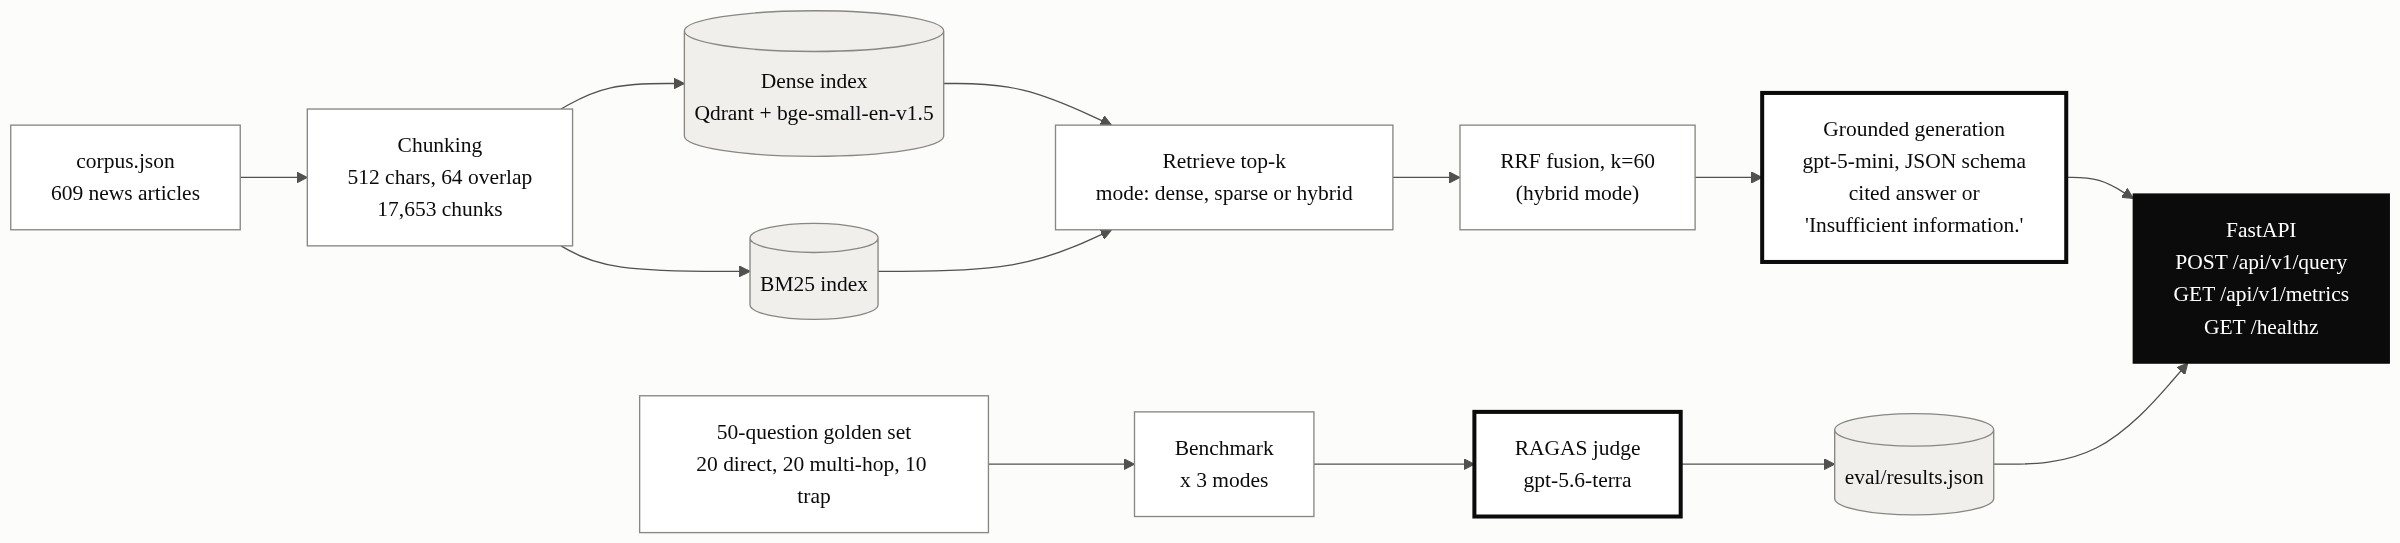
\includegraphics[width=\textwidth]{architecture.png}
\caption{System overview. Top: documents are split into chunks and stored in two indexes; a question is searched in one of three modes and answered by the LLM from the top 5 chunks. Bottom: the 50-question test set is run through all three modes and scored by a separate judge model. Thick borders mark steps that call an LLM.}
\label{fig:arch}
\end{figure*}

\textbf{1. Chunking.} Articles are too long to search as a whole, so each one is split into \term{chunks} of at most 512 characters, with 64 characters of overlap between neighbours so that a sentence cut at a boundary still appears complete in one chunk. This gave \textbf{17,653 chunks}. Each chunk gets a stable ID (a hash of its URL, position and text), so the same chunk always has the same ID.

\textbf{2. Two indexes.} All chunks are embedded and stored in Qdrant, a vector database (dense index), and also stored in a BM25 index (sparse index). Both are built from the exact same chunks, and the build fails if their ID lists differ, so the three search modes are always comparing the same material.

\textbf{3. Search modes.} \emph{Dense} returns the chunks closest in meaning; \emph{sparse} returns the best BM25 matches; \emph{hybrid} takes the top 50 from each and merges them with RRF ($k=60$, the standard default, not tuned). Each mode passes its top $k=5$ chunks to the LLM.

\textbf{4. Grounded answer.} The LLM (\code{gpt-5-mini}) gets the question and the 5 chunks, each labelled with its ID. Its instructions are strict: use only the given text, cite chunk IDs, and if the answer is not there, reply exactly ``\textbf{Insufficient information.}'' The reply must follow a fixed JSON format (answer + list of cited IDs); a malformed reply raises an error instead of being shown, and any cited ID that was not among the 5 chunks is removed and logged.

\textbf{5. Serving.} A FastAPI web service exposes the pipeline (\code{/api/v1/query}), the saved benchmark results and a health check. The whole stack starts with one Docker command (Appendix~\ref{app:repro}).

%=====================================================
\section{Experimental Setup}

\subsection{Test set}
I sampled 50 questions from the 2,556 in MultiHop-RAG with a fixed random seed (42), so the set can be rebuilt exactly:

\begin{itemize}
\item \textbf{20 ``direct''} questions (10 about timing, 10 comparisons between articles). 19 of the 20 have a yes/no-style answer.
\item \textbf{20 multi-hop} questions that require combining facts, typically to identify a person or company.
\item \textbf{10 trap} questions whose answer is \emph{not} in the collection. The only correct reply is ``Insufficient information.''
\end{itemize}

For every answerable question I located the chunks that contain its evidence facts (exact text match, with a fuzzy-match fallback for 2 facts). All 120 evidence facts were found. Each answerable question needs \textbf{2 to 5 chunks}, usually from different articles.

I started with 25 questions but increased this to 50 because, with only 20 scored questions, a single question moves an average by 5 points. I did not go to 100 because of budget (about \$9 per full run, from a student budget).

\subsection{Metrics}\label{sec:metrics}
The four RAGAS metrics are computed by a judge LLM, on a 0--1 scale, higher is better:

\begin{itemize}
\item \term{Faithfulness}: are the claims in the answer supported by the retrieved chunks? (Measures made-up content.)
\item \term{Answer relevance}: does the answer actually address the question? A refusal scores 0.
\item \term{Context precision}: are the useful chunks ranked near the top of the 5?
\item \term{Context recall}: does the retrieved text contain the information in the reference answer? (Did search find what was needed?)
\end{itemize}

Three more measures need no judge:

\begin{itemize}
\item \term{Trap refusal}: out of the 10 trap questions, how many got exactly ``Insufficient information.''
\item \term{False refusal}: out of the 40 answerable questions, how many were refused anyway.
\item \term{Latency}: time per question, mean and 95th percentile (the time 95\% of questions stay under).
\end{itemize}

\textbf{Why traps are scored separately.} RAGAS gives a refusal 0 for answer relevance, even when refusing is the correct behaviour. Averaging traps in would punish the system for being honest. So RAGAS averages use only the 40 answerable questions, and traps get their own exact-text check. (I considered telling the judge which questions are traps, but that would leak the answer to the judge.)

\subsection{Models and cost}
Generator: \code{gpt-5-mini}. Judge: \code{gpt-5.6-terra}, a different and stronger model, so the generator does not grade its own work. Search is fixed at $k=5$. Each mode ran all 50 questions one at a time (150 generations, 0 errors), and the judge produced all 480 scores (40 questions $\times$ 4 metrics $\times$ 3 modes) with none missing. The judge cost about \textbf{\$3.64} (measured from token counts) and generation roughly \$0.25 (an estimate).

%=====================================================
\section{Results}

\begin{table*}[t]
\centering
\small
\begin{tabular}{lcccccc}
\toprule
Mode & Faithfulness & Answer relevance & Context precision & Context recall & Trap refusal & Latency mean / p95 \\
\midrule
Dense  & \textbf{0.427} & 0.258 & 0.604 & 0.525 & 8/10 & 10.8\,s / 21.1\,s \\
Sparse & 0.415 & 0.211 & 0.567 & 0.550 & \textbf{9/10} & \textbf{10.0\,s / 17.0\,s} \\
Hybrid & 0.365 & \textbf{0.286} & \textbf{0.618} & \textbf{0.625} & \textbf{9/10} & 12.1\,s / 21.2\,s \\
\bottomrule
\end{tabular}
\caption{Main results. RAGAS scores are averages over the 40 answerable questions (0--1, higher is better). Trap refusal is out of the 10 unanswerable questions. Latency covers all 50 questions (lower is better). Bold = best in column. $k=5$, generator \code{gpt-5-mini}, judge \code{gpt-5.6-terra}.}
\label{tab:main}
\end{table*}

Table~\ref{tab:main} and Figure~\ref{fig:ragas} give the main numbers.

\begin{figure}[t]
\centering
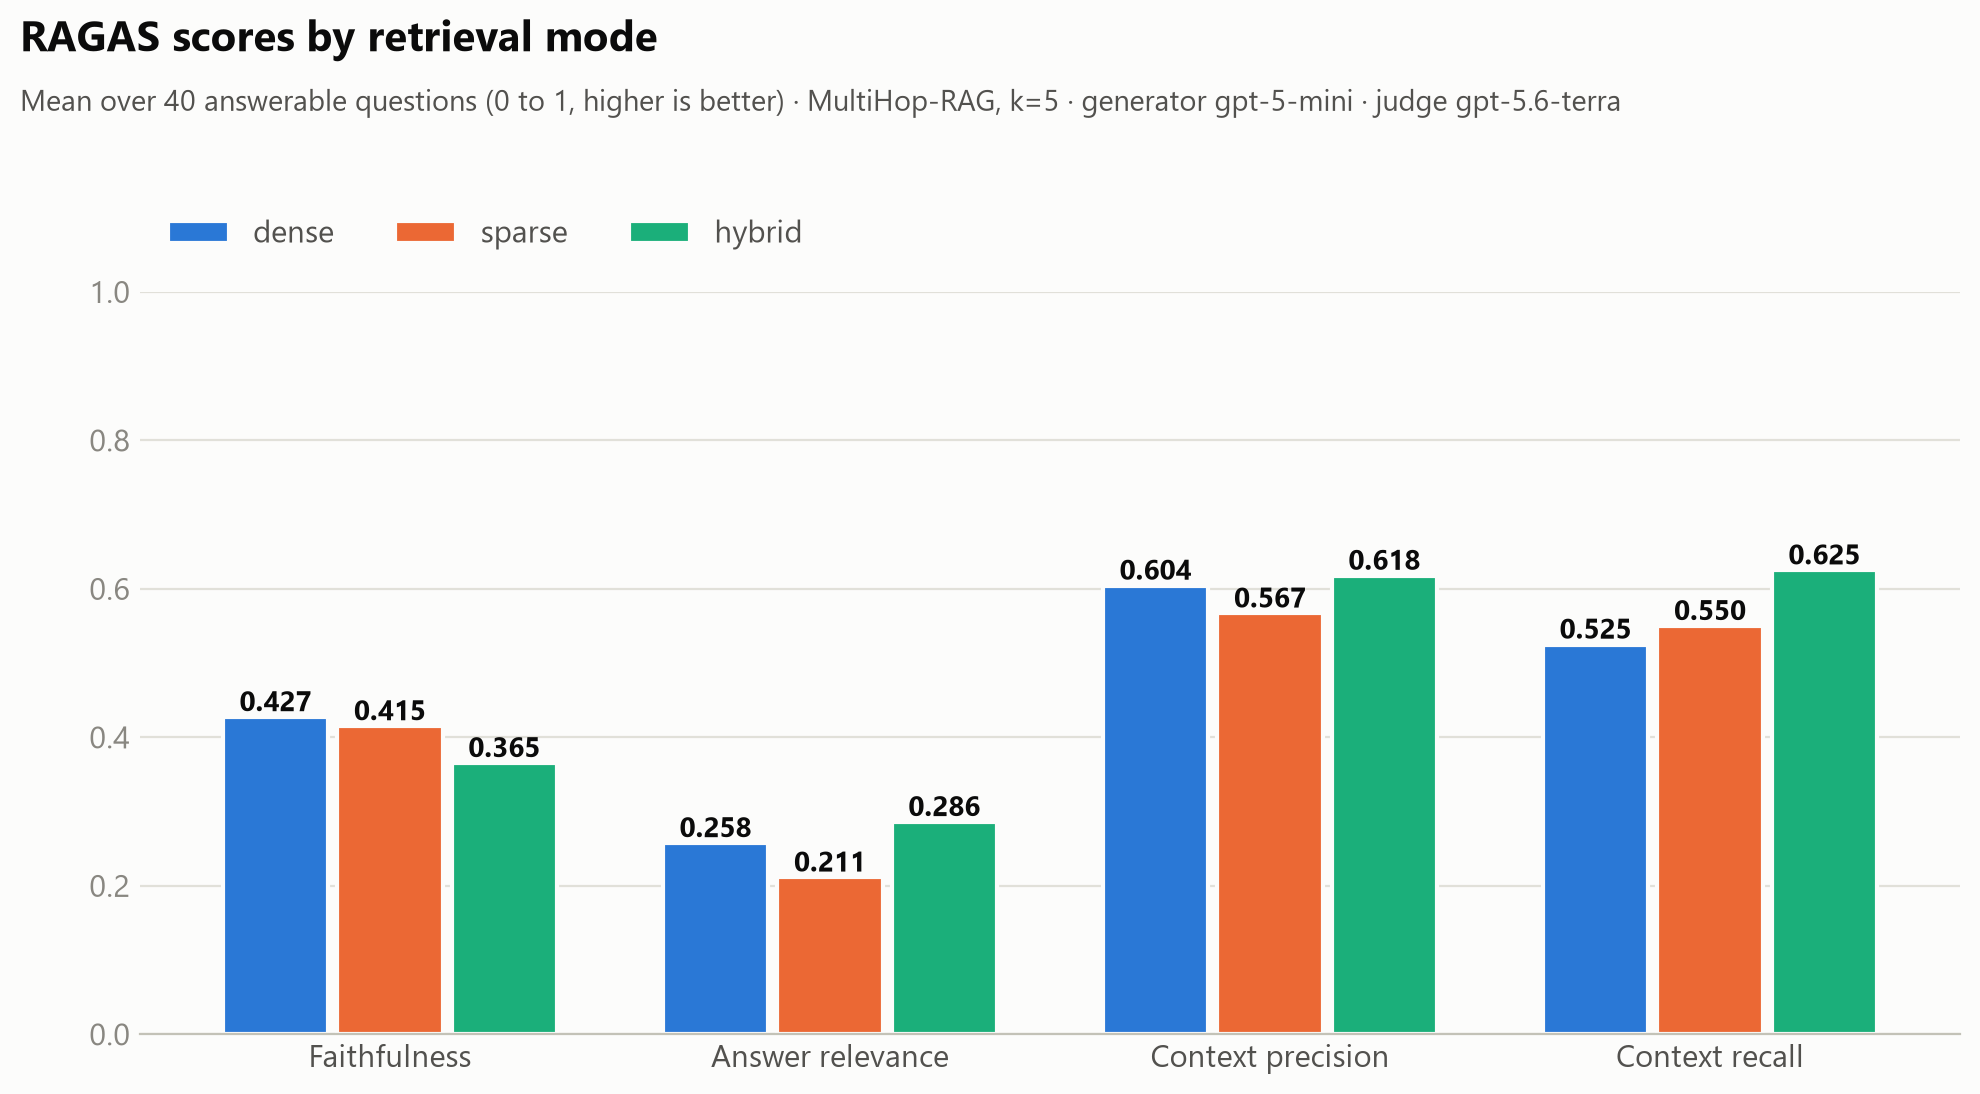
\includegraphics[width=\columnwidth]{02_ragas_metrics.png}
\caption{RAGAS scores per search mode (40 answerable questions).}
\label{fig:ragas}
\end{figure}

\textbf{Hybrid found the most evidence.} Hybrid had the best context recall (0.625 vs.\ 0.525 dense and 0.550 sparse), the best context precision and the best answer relevance. This is the direction the research question expected.

\textbf{Is the difference real?} With only 40 questions, small gaps can be luck. I ran a \term{paired bootstrap}: resample the 40 questions with replacement 10,000 times, and each time compute the hybrid-minus-dense difference on the same questions. Result: \textbf{+0.100, 95\% interval [0.000, +0.225]}. Hybrid was ahead in 94\% of resamples; per question it scored higher on 5, lower on 1 and the same on 34. Against sparse the interval is [$-$0.050, +0.200], which includes zero. \emph{In plain words: the evidence leans toward hybrid, but 40 questions are not enough to be sure.}

\textbf{Faithfulness was lowest for hybrid} (0.365). As Section~\ref{sec:lowscores} shows, averages here are dominated by refusals, so this should not be over-read.

\textbf{Trick questions.} All modes refused 8 or 9 of the 10 traps (Figure~\ref{fig:refusal}). A one-question difference is not a ranking.

\begin{figure}[t]
\centering
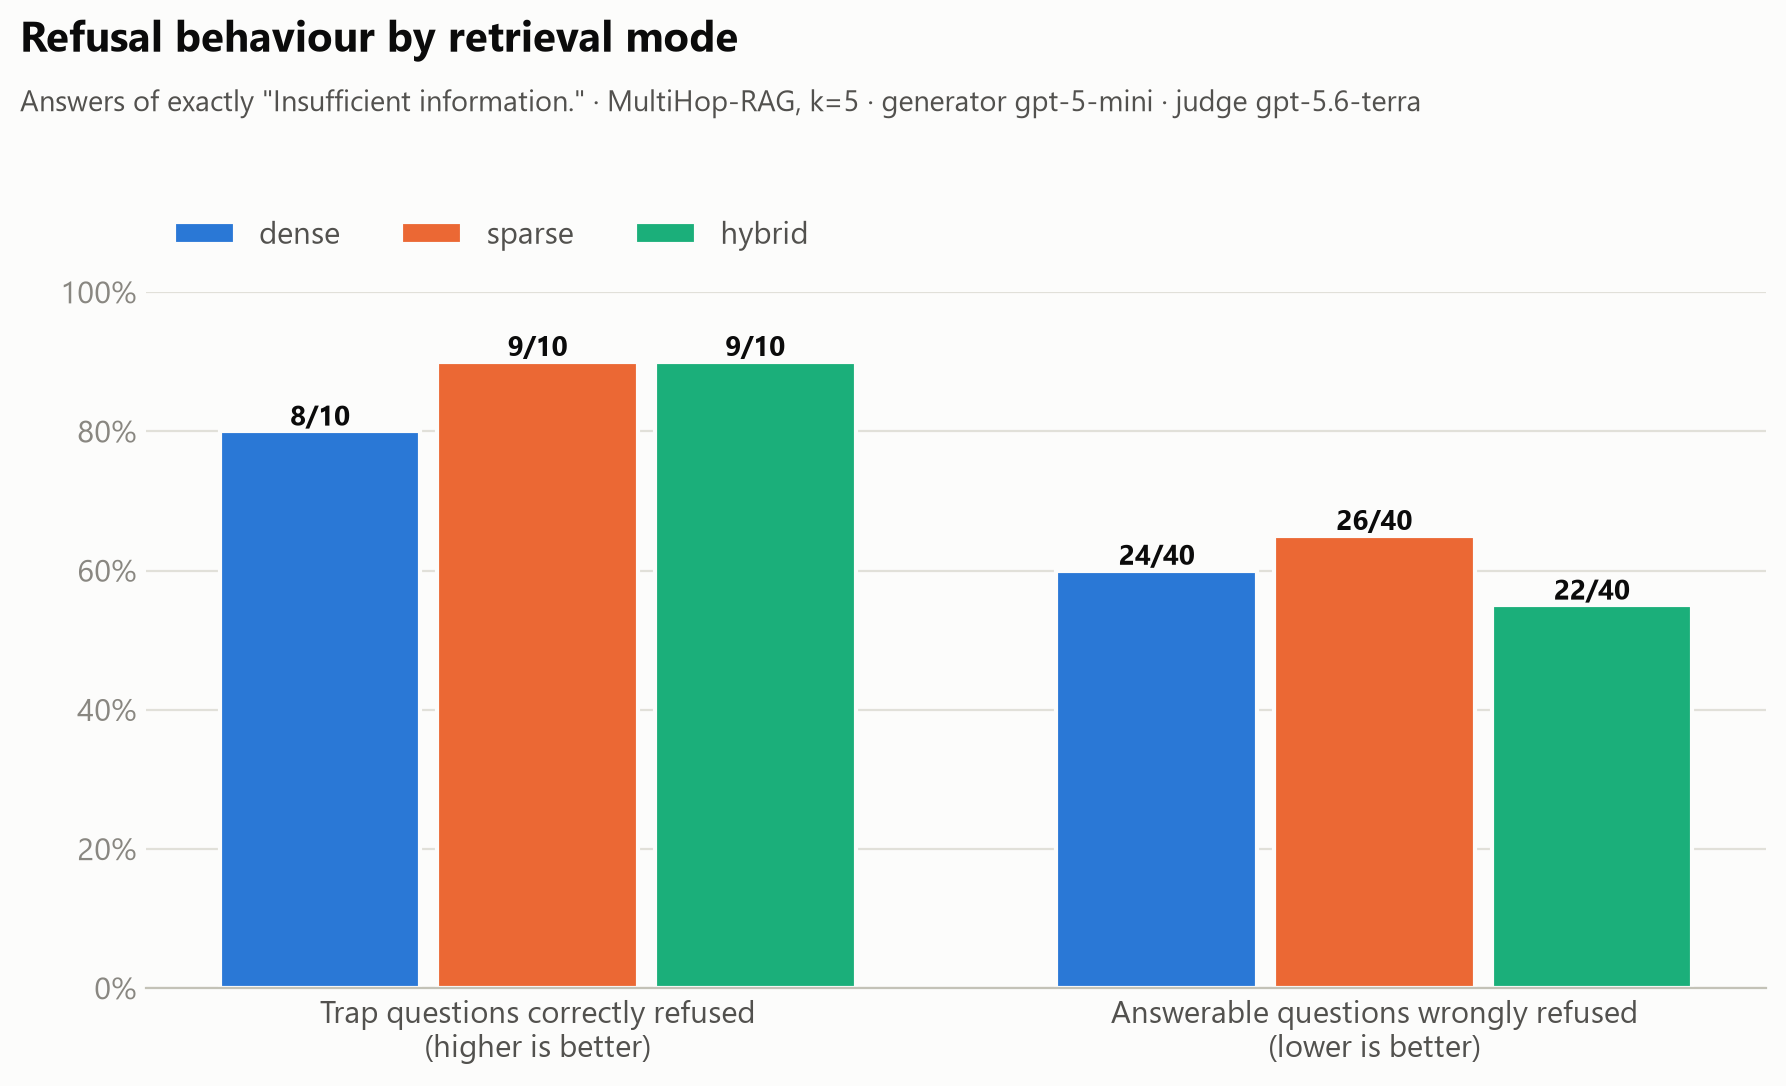
\includegraphics[width=\columnwidth]{03_refusal_behavior.png}
\caption{Refusals. Left: trap questions correctly refused (higher is better). Right: answerable questions wrongly refused (lower is better).}
\label{fig:refusal}
\end{figure}

\textbf{The surprise: too many refusals.} The model said ``Insufficient information.'' on \textbf{22 to 26 of the 40 answerable questions} (55--65\%). The next section explains why.

%=====================================================
\section{Analysis}

\subsection{Search, not the LLM, is the bottleneck}
Because I know which chunks hold each question's evidence, I can check how many of them made it into the top 5, with no LLM involved (Figure~\ref{fig:evidence}).

\begin{figure}[t]
\centering
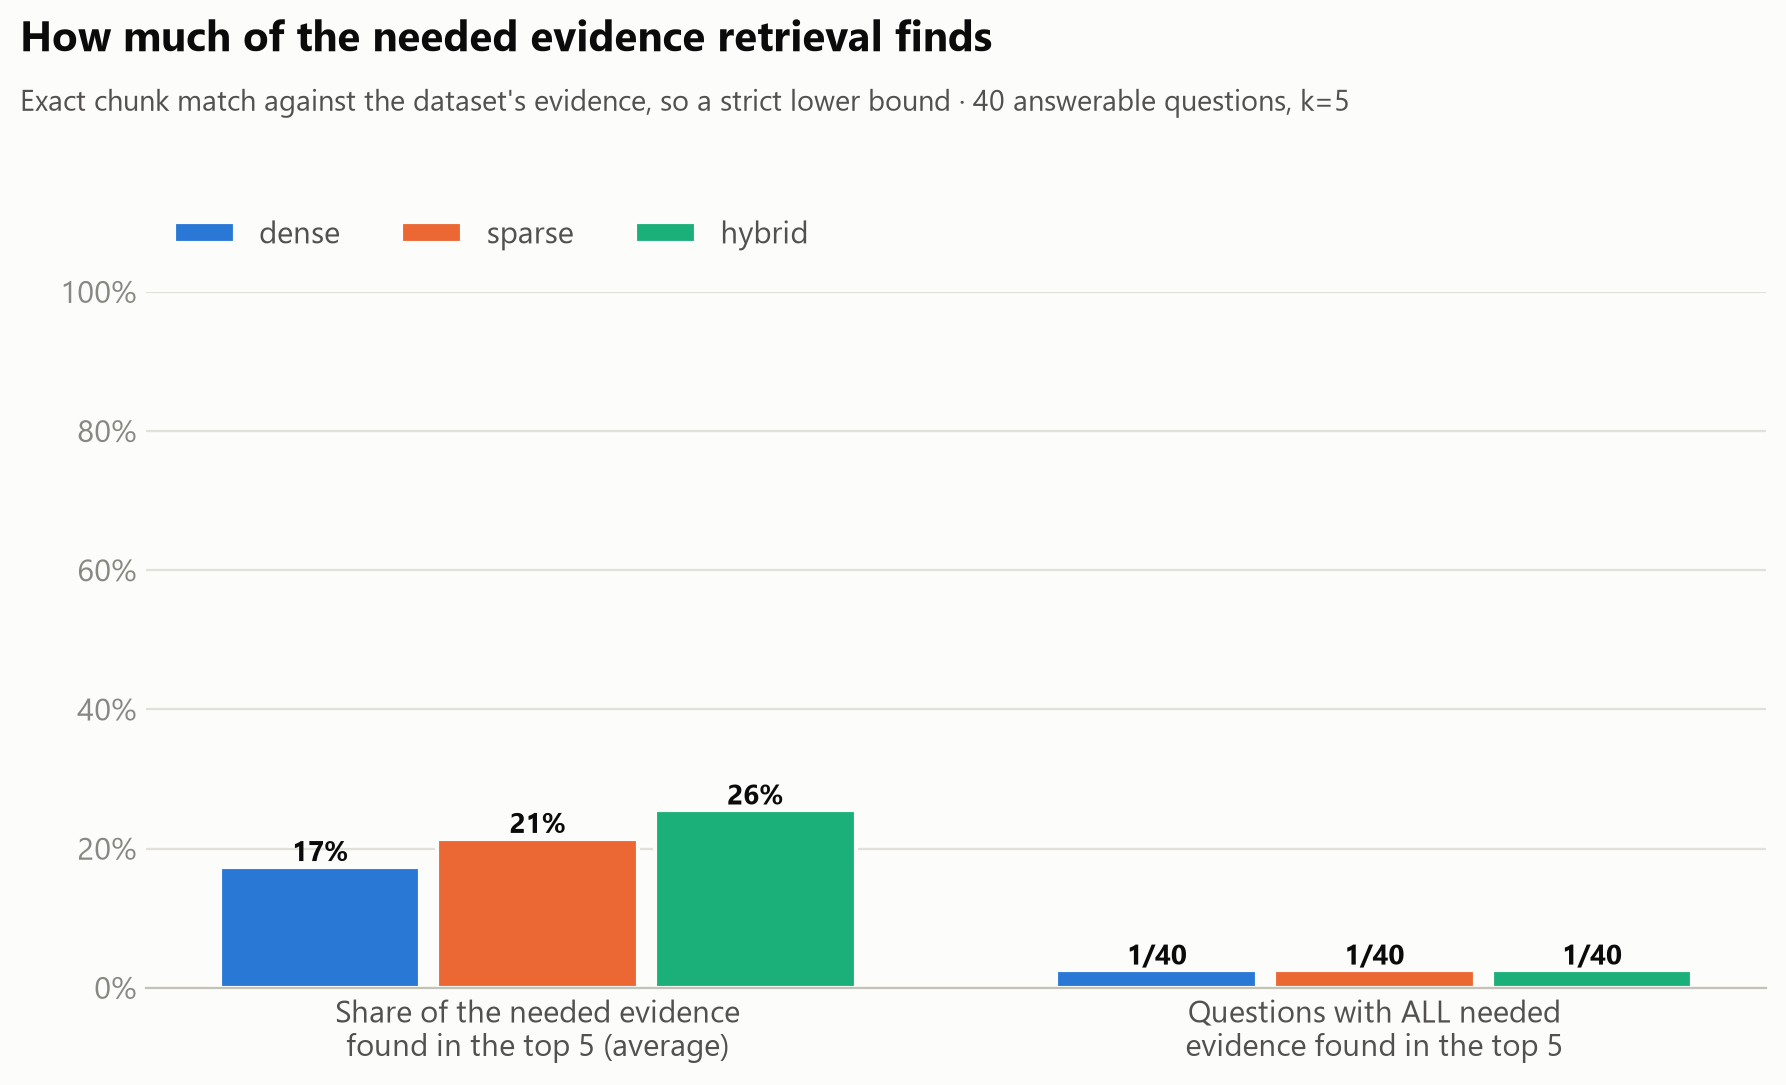
\includegraphics[width=\columnwidth]{05_evidence_retrieved.png}
\caption{Share of the needed evidence chunks that search placed in the top 5. Only 1 of 40 questions had all its evidence found, in every mode.}
\label{fig:evidence}
\end{figure}

On average the top 5 held only \textbf{17\% (dense), 21\% (sparse) and 26\% (hybrid)} of the needed evidence chunks, and only \textbf{1 of 40} questions had \emph{all} of its evidence retrieved. Figure~\ref{fig:outcomes} links this to the refusals: in hybrid mode, of the 22 refused answerable questions, 11 had none of their evidence, 11 had only part of it, and \textbf{none had all of it}. Across all three modes there was only one refusal where everything needed was actually retrieved (sparse).

\begin{figure*}[t]
\centering
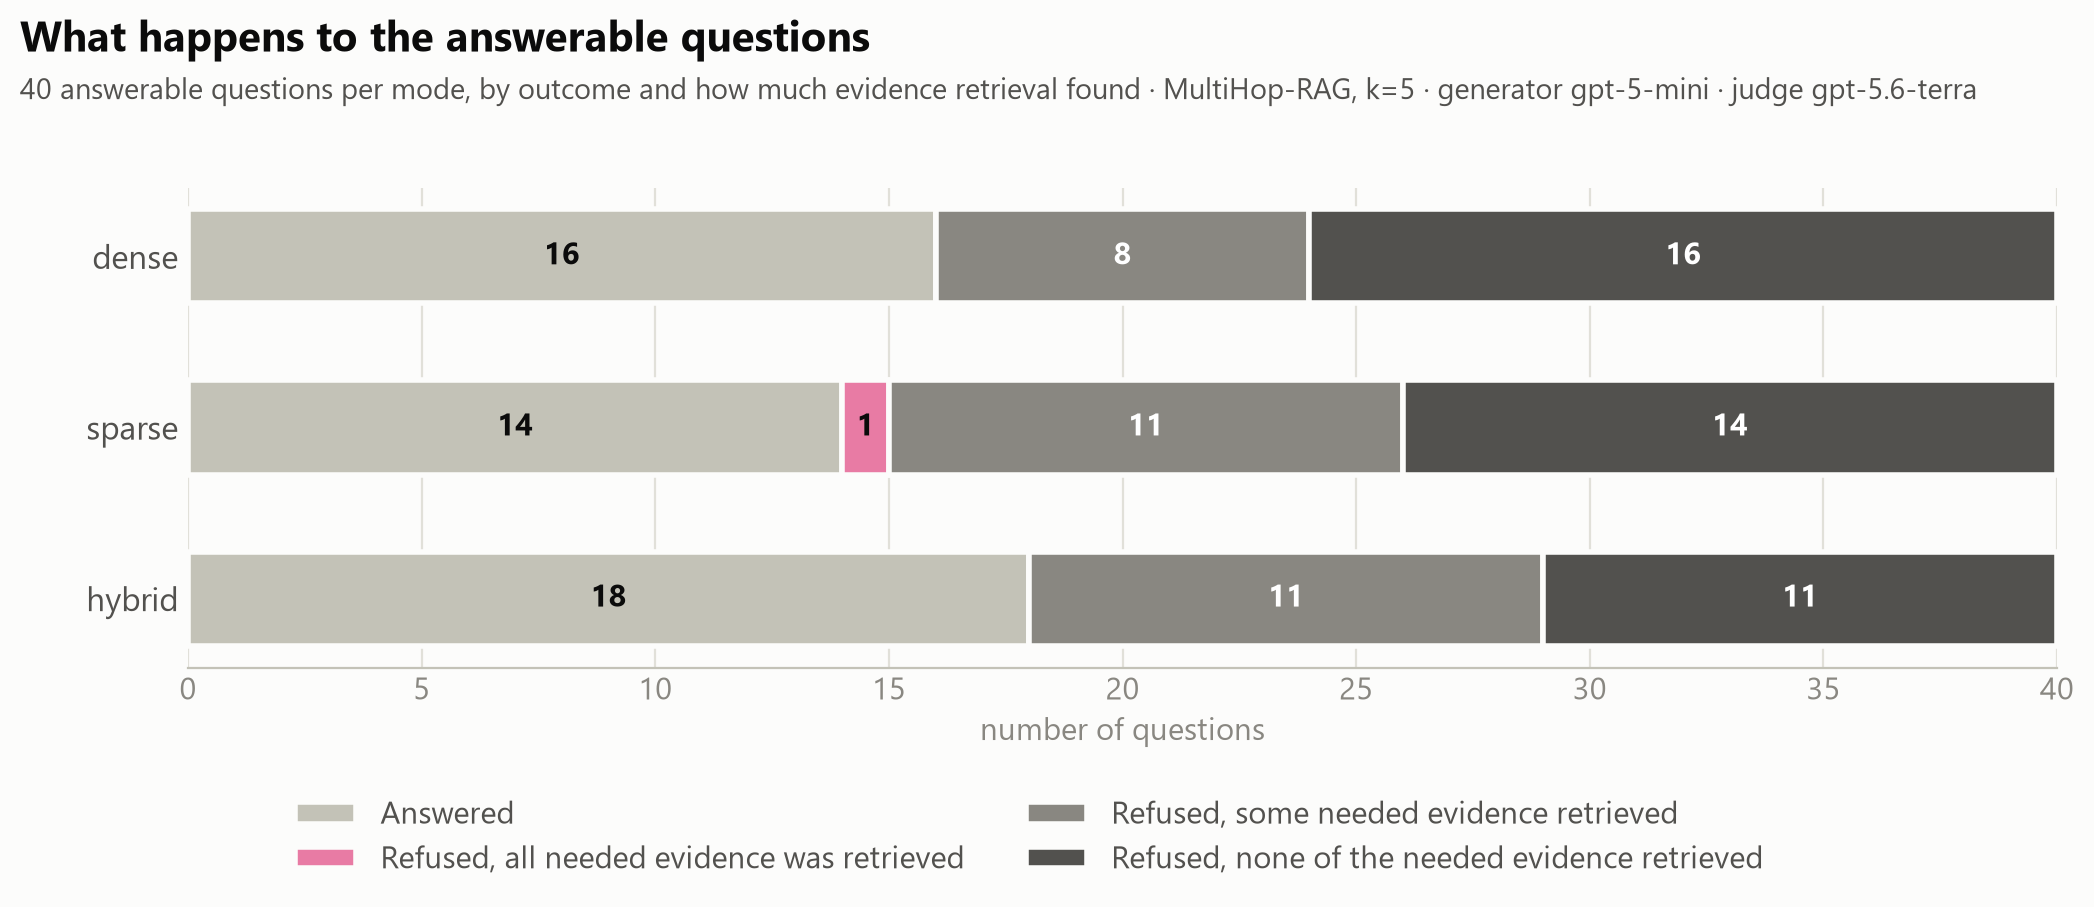
\includegraphics[width=0.82\textwidth]{06_answerable_outcomes.png}
\caption{What happened to the 40 answerable questions in each mode, split by how much of the needed evidence search found. Almost every refusal happened when evidence was missing.}
\label{fig:outcomes}
\end{figure*}

So the refusals are mostly \emph{correct} behaviour: the LLM followed its rule and did not guess when the evidence was missing. The problem is upstream, in search. Hybrid refused the least (22) because it found the most evidence.

\subsection{Why the RAGAS averages look low}\label{sec:lowscores}
Splitting the scores by outcome makes the picture clear. On questions the model \emph{answered}, scores were reasonable: faithfulness 0.59--0.69, answer relevance 0.60--0.64, context precision 0.71--0.88, context recall 0.75--1.00. On refused questions, answer relevance is exactly 0 by definition and faithfulness was only 0.18--0.27. Since more than half the questions were refused, they pull every average down.

One caution: the ``answered'' questions are a different set in each mode, so answered-only numbers must not be compared across modes. The fair comparison remains the 40-question average in Table~\ref{tab:main}.

\subsection{A concrete failure: question q11}
q11 asks whether a \emph{Fortune} article and a \emph{TechCrunch} article describe the Israel conflict in a certain way. In hybrid mode, all 5 retrieved chunks came from the TechCrunch article and none from Fortune. A comparison was impossible, so refusing was right. This is the typical multi-hop failure: \textbf{the top 5 fills up with chunks from one article}, and the second source never gets a place.

\subsection{When the model did not refuse a trap}
The few non-refused traps are real hallucinations, and they share a pattern. Trap q47 asks which baseball position ``represented by a single character'' a baseball executive prioritized; all three modes gave an answer built around the number ``5'', with a citation. Trap q48 asks for the first letter of a new MacBook Pro feature; dense answered ``M'', taken from an article about Apple's M3 chips. In both cases the question looked answerable, the retrieved text contained something related, and the model produced a confident, cited, but unsupported answer. Citations alone do not prove grounding.

\subsection{Where the time goes}
Mean latency was 10--12\,s per question (Figure~\ref{fig:latency}). To find out why, I ran the real web service with the LLM replaced by a fake: the whole endpoint (search, fusion, building the response) took only \textbf{38\,ms (dense), 50\,ms (sparse) and 83\,ms (hybrid)}. So more than 99\% of the time is the LLM. \code{gpt-5-mini} is a ``reasoning'' model that thinks before answering; with \code{gpt-4o-mini} the same question took about 1\,s. Hybrid's extra cost is real but tiny (about 45\,ms more than dense).

\begin{figure}[t]
\centering
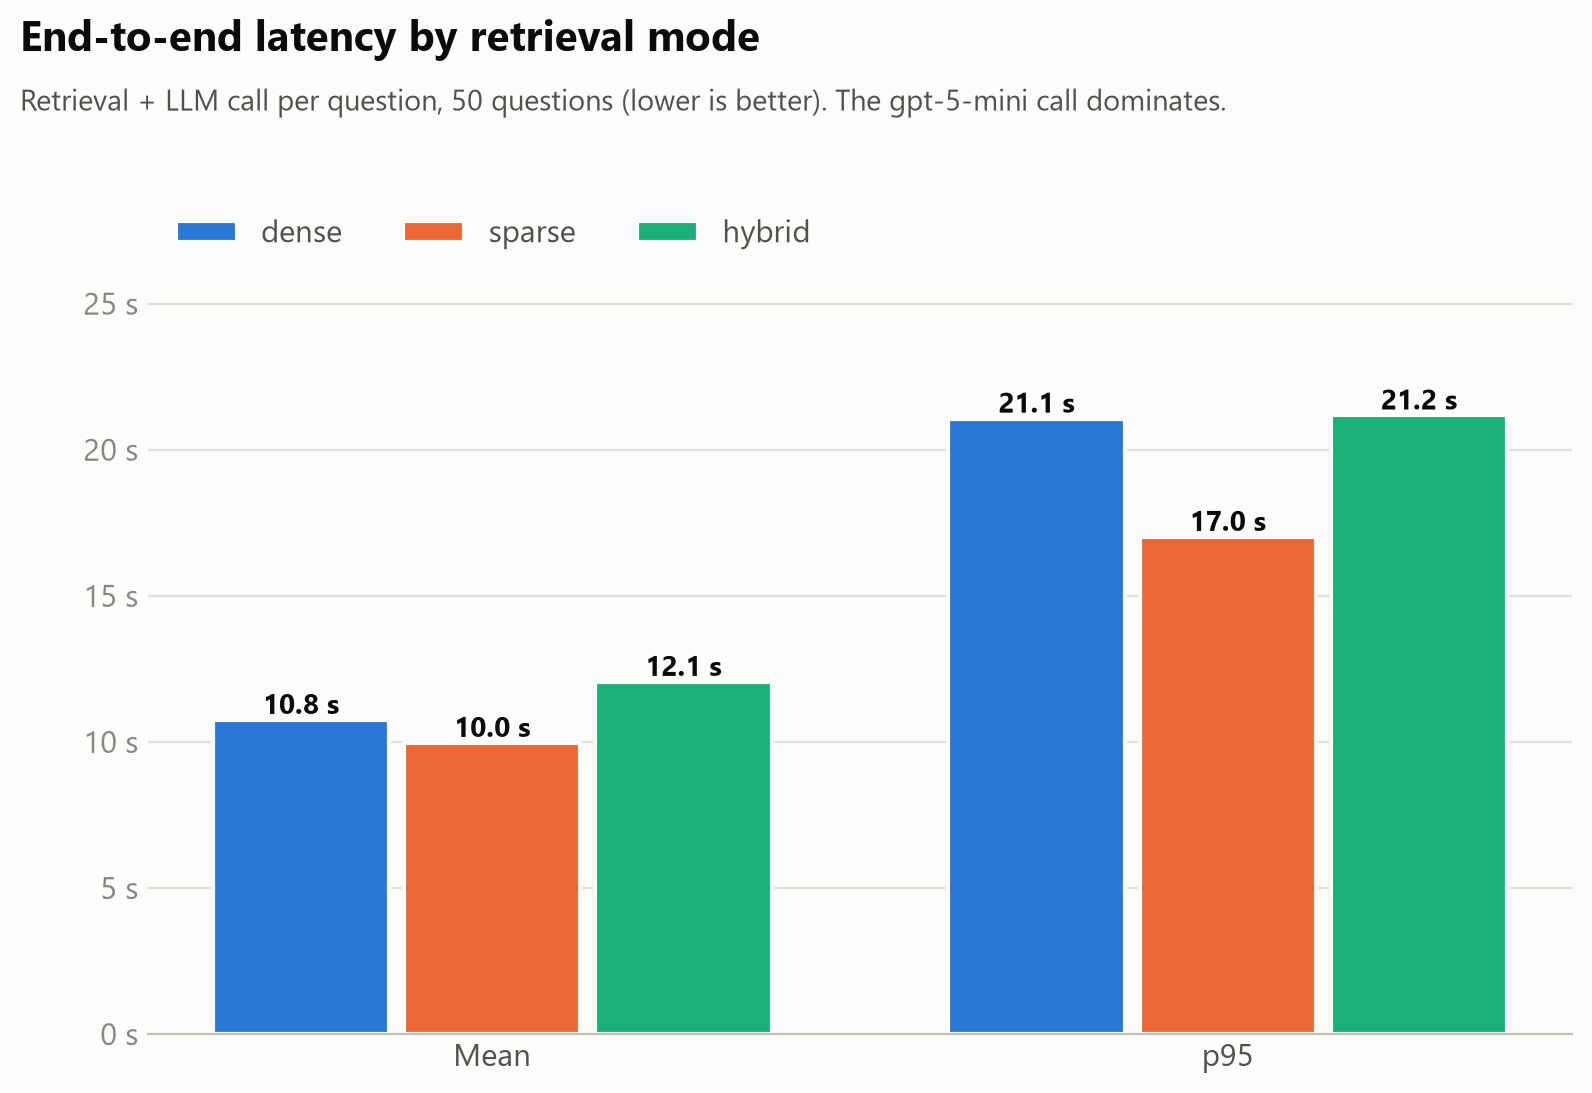
\includegraphics[width=0.92\columnwidth]{04_latency.png}
\caption{Latency per question, including the LLM call.}
\label{fig:latency}
\end{figure}

\subsection{A weakness of RRF seen during testing}
For a long paraphrased question about the game \emph{Cocoon}, dense search ranked the correct chunk \#1, but BM25 did not have it in its top 50. Its RRF score was only $1/61 = 0.016$. A mediocre chunk ranked \#44 by dense and \#2 by BM25 scored $1/104 + 1/62 = 0.026$ and pushed the correct chunk out of the hybrid top 5. RRF rewards agreement between the two lists over one confident list. This is one reason hybrid is not always better, and it suggests tuning $k$ or weighting the lists.

%=====================================================
\section{Limitations}
\begin{itemize}
\item \textbf{Small sample.} 40 scored questions give wide confidence intervals; differences of 0.05--0.10 are within noise.
\item \textbf{Narrow question types.} 19 of 20 direct questions are yes/no, and 9 of 20 multi-hop answers are the same person (Sam Bankman-Fried), so the set covers fewer topics than its size suggests.
\item \textbf{No correctness metric.} None of the four RAGAS metrics compares the answer with the reference answer.
\item \textbf{Judge bias.} Generator and judge are both OpenAI models, so some same-vendor bias is possible.
\item \textbf{Not exactly repeatable.} \code{gpt-5-mini} and the judge do not allow setting temperature to 0, so a rerun gives slightly different numbers. The benchmark was run once.
\item \textbf{Strict evidence check.} Only the exact evidence chunk counts as found; a different chunk with the same fact does not. The 17--26\% figures are therefore a lower bound.
\item \textbf{Default settings.} Chunk size, overlap, RRF $k$, the 50-candidate pool and the embedding model were all left at defaults.
\end{itemize}

%=====================================================
\section{Future Work}
Each item below is a hypothesis to test, not a result.

\begin{center}
\small
\begin{tabularx}{\columnwidth}{@{}>{\raggedright\arraybackslash}p{0.33\columnwidth}>{\raggedright\arraybackslash}X@{}}
\toprule
Idea & Why it might help \\
\midrule
Larger $k$ (10, 20) & Multi-hop questions need 2--5 chunks from different articles; 5 slots rarely hold them all. \\
Diversify results (max chunks per article, or MMR \cite{mmr}) & Stops one article from filling the top 5 (the q11 failure). \\
Query decomposition & Split a two-source question into one search per source, then merge. \\
Recall@$k$ on known chunks & Measures search alone, with no judge cost. \\
Cross-encoder reranker, tuned RRF & Re-scores candidates more carefully; fixes cases like Cocoon. \\
More questions, repeated runs & Tighter intervals and a measure of run-to-run spread. \\
Answer-correctness metric, cross-vendor judge & Checks the answer itself and reduces judge bias. \\
Stricter grounding check & A second pass to catch cited-but-unsupported answers (q47, q48). \\
\bottomrule
\end{tabularx}
\end{center}

The first two are the most promising, because the analysis shows that missing evidence is the main problem.

%=====================================================
\section{Conclusion}
I built a complete, measured RAG pipeline and compared dense, sparse and hybrid search on the same multi-hop questions. Hybrid search found the most evidence and refused the fewest answerable questions, but with 40 questions its advantage is suggestive rather than proven. The clearest lesson came from measuring beyond the headline scores: the LLM behaved well, refusing when evidence was missing, while search delivered only about a fifth of the needed evidence. For multi-hop questions, improving \emph{what reaches the model} (more and more varied results) is the next step, and this setup can now measure whether it works.

%=====================================================
\small
\begin{thebibliography}{99}
\setlength{\itemsep}{1pt}
\bibitem{lewis} P. Lewis et al. Retrieval-Augmented Generation for Knowledge-Intensive NLP Tasks. \emph{NeurIPS}, 2020. arXiv:2005.11401.
\bibitem{gao} Y. Gao et al. Retrieval-Augmented Generation for Large Language Models: A Survey. arXiv:2312.10997, 2023.
\bibitem{manning} C. D. Manning, P. Raghavan, H. Sch\"utze. \emph{Introduction to Information Retrieval}. Cambridge University Press, 2008.
\bibitem{robertson} S. Robertson, H. Zaragoza. The Probabilistic Relevance Framework: BM25 and Beyond. \emph{Foundations and Trends in IR}, 2009.
\bibitem{dpr} V. Karpukhin et al. Dense Passage Retrieval for Open-Domain Question Answering. \emph{EMNLP}, 2020. arXiv:2004.04906.
\bibitem{bge} S. Xiao et al. C-Pack: Packaged Resources To Advance General Chinese Embedding. arXiv:2309.07597, 2023.
\bibitem{beir} N. Thakur et al. BEIR: A Heterogeneous Benchmark for Zero-shot Evaluation of Information Retrieval Models. \emph{NeurIPS Datasets and Benchmarks}, 2021. arXiv:2104.08663.
\bibitem{rrf} G. V. Cormack, C. L. A. Clarke, S. B\"uttcher. Reciprocal Rank Fusion Outperforms Condorcet and Individual Rank Learning Methods. \emph{SIGIR}, 2009.
\bibitem{ragas} S. Es et al. RAGAS: Automated Evaluation of Retrieval Augmented Generation. arXiv:2309.15217, 2023.
\bibitem{multihop} Y. Tang, Y. Yang. MultiHop-RAG: Benchmarking Retrieval-Augmented Generation for Multi-Hop Queries. \emph{COLM}, 2024. arXiv:2401.15391.
\bibitem{mmr} J. Carbonell, J. Goldstein. The Use of MMR, Diversity-Based Reranking for Reordering Documents and Producing Summaries. \emph{SIGIR}, 1998.
\end{thebibliography}
\normalsize

%=====================================================
\appendix
\section{Reproducibility}\label{app:repro}
\textbf{Code:} the \code{eval-hybrid-rag} repository (Python 3.13, dependencies locked with \code{uv}). \textbf{Data:} MultiHop-RAG (ODC-BY licence). \textbf{Test set:} 50 questions, seed 42, saved in \code{eval/test\_dataset.json}. \textbf{Summary results:} \code{eval/results.json}.

\begin{itemize}
\item \code{docker compose up --build}: downloads data, builds both indexes, starts the API (about 20 minutes on an 8-core CPU from an empty start; under a minute afterwards).
\item \code{uv run python -m eval.benchmark}: full benchmark (about \$4, 30+ minutes).
\item \code{uv run python -m eval.make\_charts}: regenerates all figures.
\item \code{uv run pytest}: 21 unit and API tests, no network or API key needed.
\end{itemize}

\section{Engineering Notes}
Real problems met while building the experiment, and how each was solved:

\begin{itemize}
\item \textbf{Text encoding on Windows.} Saving the dataset crashed on special characters (such as emoji) because Windows used a Hebrew codepage by default. Fixed by forcing UTF-8 everywhere.
\item \textbf{A silent hang in the judge.} The judge model only accepts its default temperature, but RAGAS always sends a near-zero value. Every call was rejected and retried, so the first test hung for minutes. Fixed with a small wrapper that removes the temperature setting; retries and timeouts were also capped.
\item \textbf{A broken dependency.} RAGAS failed to import because a newer \code{langchain-community} removed a module it needs, and it also needed Pillow without declaring it. Found by testing in a throwaway environment first, then pinning the working versions.
\item \textbf{Keeping cost under control.} The benchmark records a failed item as an error and continues, instead of crashing halfway through a paid run. Judge cost was measured on 3 samples before the full run (about \$0.03 per scored answer), which set the test-set size.
\item \textbf{A smaller Docker image.} The first dependency lock pulled 43 GPU packages (several GB) that a CPU server never uses. Switching Linux to CPU-only PyTorch and keeping evaluation tools out of the image gave a 2.64\,GB image; the running API uses about 590\,MB of memory.
\item \textbf{Clear errors.} Without an API key, the query endpoint returned a bare ``500 Internal Server Error''. It now returns a 503 with a message that explains what is missing. A test from a completely clean copy of the repository confirmed the one-command start works.
\end{itemize}

\end{document}
